\documentclass{article}
\usepackage[utf8]{inputenc}
\usepackage[T1]{fontenc}
\usepackage[french]{babel}

% ------------------------- Color table ----------------------------------------
\usepackage{multirow}
\usepackage[table]{xcolor}
\definecolor{maroon}{cmyk}{0,0.87,0.68,0.32}
% ------------------------------------------------------------------------------

\usepackage{amscd}
\usepackage{amsthm}
\usepackage{physics}
\usepackage[left=2.2cm,right=2.2cm,top=2cm,bottom=2cm]{geometry}
\usepackage{textcomp,gensymb} %pour le °C, et textcomp pour éviter les warning
\usepackage{graphicx} %pour les images
\usepackage{caption}
\usepackage{subcaption}
\usepackage[colorlinks=true,
	breaklinks=true,
	citecolor=blue,
	linkcolor=blue,
	urlcolor=blue]{hyperref} % pour insérer des liens
\usepackage{epstopdf} %converting to PDF
\usepackage[export]{adjustbox} %for large figures

\usepackage{array}
\usepackage{dsfont}% indicatrice : \mathds{1}


% -------------------------- Mathematics ---------------------------------------
\graphicspath{{images/}{../images/}} % For the images path
% ------------------------------------------------------------------------------

% -------------------------- Mathematics ---------------------------------------
\usepackage{mathrsfs, amsmath, amsfonts, amssymb}
\usepackage{bm}
\usepackage{mathtools}
\usepackage[Symbol]{upgreek} % For pi \uppi different from /pi
\newcommand{\R}{\mathbb{R}} % For Real space

% ------------------------------------------------------------------------------


% -------------------------- Code format ---------------------------------------
\usepackage[numbered,framed]{matlab-prettifier}
\lstset{
	style              = Matlab-editor,
	basicstyle         = \mlttfamily,
	escapechar         = '',
	mlshowsectionrules = true,
}
% ------------------------------------------------------------------------------

% ------------------------- Blbiographie --------------------------------------
\usepackage[backend=biber, style=ieee]{biblatex}
\addbibresource{biblio.bib}
% ------------------------------------------------------------------------------


\setcounter{tocdepth}{4} %Count paragraph
\setcounter{secnumdepth}{4} %Count paragraph
\usepackage{float}

\usepackage{graphicx} % for graphicspath
% \graphicspath{{../images/}}

\usepackage{array,tabularx}
\newcolumntype{L}[1]{>{\raggedright\let\newline\\\arraybackslash\hspace{0pt}}m{#1}}
\newcolumntype{C}[1]{>{\centering\let\newline\\\arraybackslash\hspace{0pt}}m{#1}}
\newcolumntype{R}[1]{>{\raggedleft\let\newline\\\arraybackslash\hspace{0pt}}m{#1}}

% to start counting section to 6


%%%%%%%%%%%%%%%%%%%%%%%%%%%%%%%%%%%%%%%%%%%
% Header
%%%%%%%%%%%%%%%%%%%%%%%%%%%%%%%%%%%%%%%%%%%

\renewcommand{\assignmenttitle}{Assignment 1: Title of the assignment}
\renewcommand{\studentname}{Vincent Matthys}
\renewcommand{\email}{vincent.matthys@ens-paris-saclay.fr}

%%%%%%%%%%%%%%%%%%%%%%%%%%%%%%%%%%%%%%%%%%%
% Syntax for using figure macros:
%%%%%%%%%%%%%%%%%%%%%%%%%%%%%%%%%%%%%%%%%%%

% \singlefig{filename}{scalefactor}{caption}{label}
% \doublefig{\subfig{filename}{scalefactor}{subcaption}{sublabel}}
%           {\subfig{filename}{scalefactor}{subcaption}{sublabel}}
%           {global caption}{label}
% \triplefig{\subfig{filename}{scalefactor}{subcaption}{sublabel}}
%           {\subfig{filename}{scalefactor}{subcaption}{sublabel}}
%           {\subfig{filename}{scalefactor}{subcaption}{sublabel}}
%           {global caption}{label}
%
% Tips:
% - with scalefactor=1, a single figure will take the whole page width; a double figure, half page width; and a triple figure, a third of the page width
% - image files should be placed in the image folder
% - no need to put image extension to include the image
% - for vector graphics (plots), pdf figures are suggested
% - for images, jpg/png are suggested
% - labels can be left empty {}

%%%%%%%%%%%%%%%%%%%%%%%%%%%%%%%%%%%%%%%%%%%
% Beginning of assignment
%%%%%%%%%%%%%%%%%%%%%%%%%%%%%%%%%%%%%%%%%%%
\begin{document}
\maketitle

\question{QIA.1: (i) Why is it important to have a similarity co-variant feature detector? (ii) How does this affect the descriptors computed at these detections? (iii) How does this affect the matching process?}

\begin{enumerate}
	\item It is important to have a similarity co-variant feature detector in order to extract the same regions of interest regardless of translations, rotations or scales, \textit{i.e.} regardless of viewpoints.
	\item The fact that the feature detector is co-variant causes the descriptors computed at these detections to be invariant after renormalisation step.
	\item Having feature detectors with similarity co-variance and feature descriptors allows the matching process to be independant of the viewpoints of the images.
\end{enumerate}

\question{QIA.2: Show the detected features in the two images for three different values of the peakThreshold option}

\triplefig{\subfig{IA_2_1}{1}{\(peakThreshold = 0.0001\)}{fig:002:th_0.0001}} % sublabels used here
{\subfig{IA_2_2}{1}{\(peakThreshold = 0.001\)}{fig:002:th_0.001}}
{\subfig{IA_2_3}{1}{\(peakThreshold = 0.01\)}{fig:002:th_0.01}}
{Feature detectors with three different values of \(peakThreshold\) for all\_souls\_000002.jpg}{fig:002}

\triplefig{\subfig{IA_2_4}{1}{\(peakThreshold = 0.0001\)}{fig:015:th_0.0001}} % sublabels used here
{\subfig{IA_2_5}{1}{\(peakThreshold = 0.001\)}{fig::015:th_0.001}}
{\subfig{IA_2_6}{1}{\(peakThreshold = 0.01\)}{fig::015:th_0.01}}
{Feature detectors with three different values of \(peakThreshold\) for all\_souls\_000015.jpg}{fig:015}

The detected features for \(peakThreshold \in \{0.0001, 0.001, 0.01\}\) are shown in Figure~\ref{fig:002} for the all\_souls\_000002.jpg image, and in Figure~\ref{fig:015} for the all\_souls\_000015.jpg image. As expected, the number of keypoints decreses with the threshold. Moreover the keypoints are fewer in the darker regions, wich leads to asymetric density in the Figure~\ref{fig:015}, especially because of the building shadow.

\question{QIA.3: Note the change in spatial density of detections across images, for a given value of peakThreshold. (i) Is the density uniform? If not, why? (ii) Which implications for image matching can this have? (iii) How can it be avoided?}
\begin{enumerate}
	\item In Figures~\ref{fig:002:th_0.0001} and~\ref{fig:015:th_0.0001}. The density is clearly not uniform between the two images. In both, the top-center of the image is very dense, but, in the first one, the grass admits no detection, which leads to a gap in the density, with some detections in the bottom limit of the grass.
	\item This can lead to error matching the correspondances with local features
	\item To avoid it we can proceed to a spatial verification relying on global geometric relations.
\end{enumerate}


\question{QIB.1: Note the descriptors are computed over a much larger region (shown in blue) than the detection (shown in green). Why is this a good strategy?}

\doublefig{\subfig{IB_2}{1}{4x4 grid arround the keypoint}{fig:4x4grid}}
{\subfig{IB_3_1}{1}{first NN match}{fig:firstNN}}
{Computation of SIFT descriptors and matching}{fig:IB1}


The larger regions are shown in Figure~\ref{fig:4x4grid}. It is a good strategy to be insensitive to small geometric deformations, and small variations of illumination, by taking the average over a larger region


\question{QIB.2: Examine carefully the mismatches and try to understand the different causes of mismatch. (i) In your report, present at least 3 of them and explain why the mistakes are being made. For example, is the change in lighting a problem? (ii) What additional constraints can be applied to remove the mismatches?}

\singlefig{IB_3}{1}{Three mismatches with SIFT features descriptors, subgroup of matches extracted from~\ref{fig:firstNN}}{fig:3miss}
\begin{enumerate}
	\item Three types of mismatch are presentend in Figure~\ref{fig:3miss}, and are extracted from Figure~\ref{fig:firstNN} \begin{itemize}
		      \item repetitive pattern (in blue)
		      \item constant local change in lighting leading to similarity between two different keypoints (in red)
		      \item ambiguity between a keypoint his first two nearest neighbors (in yellow)
	      \end{itemize}
	      A global change in lighting is irrelevant for matching, because of the gradient nullifying the constant component
	\item Geometric verification with global constraints can discard those mismatches. Another method, presented below, is to look at the second nearest neigbour to remove ambiguous matches.
\end{enumerate}

\question{QIC.1: Illustrate and comment on improvements that you can achieve with this step. Include in your report figures showing the varying number of tentative matches when you change the nnThreshold parameter.}

As expected, the percentage of matches kept increases with \( nnThreshold\). The results obtained are shown in Figures~\ref{fig:IC_12}~\ref{fig:IC_34}~\ref{fig:IC_5}. Until \( nnThreshold = 0.7\), there is no substantial mismatches, but the number of matches kept is below \( 10~\%\). If more matches are kept, a non-negligeable part of new matches is missmatches, because the ambiguity between the first and the second nearest neighbour is no longer removed. In Figure~\ref{fig:graphnnth} we can see the exponential growth of the number of matches with \( nnThreshold \). A good compromise would be to take the threshold before this exponential growth.

\doublefig{\subfig{IC_1}{1}{\( nnThreshold = 0.3\)}{fig:nth0.3}}
{\subfig{IC_2}{1}{\( nnThreshold = 0.5\)}{fig:nth0.5}}
{Matching using Lowe's second nearest neighbour - part1}{fig:IC_12}
\doublefig{\subfig{IC_3}{1}{\( nnThreshold = 0.7\)}{fig:nth0.7}}
{\subfig{IC_4}{1}{\( nnThreshold = 0.9\)}{fig:nth0.9}}
{Matching using Lowe's second nearest neighbour - part2}{fig:IC_34}
\doublefig{\subfig{IC_5}{1}{\( nnThreshold = 0.8\)}{fig:nth0.8}}
{\subfig{2nn_graph}{1}{Percentage of matches in function of the \( nnThreshold\)}{fig:graphnnth}}
{Matching using Lowe's second nearest neighbour - part3}{fig:IC_5}


\question{QID.1: Work out how to compute this transformation from a single correspondence. Hint: recall from Stage I.A that a SIFT feature frame is an oriented circle and map one onto the other.}
We need four equations to compute the transformation. With a signle correspondance, we can have 2 equations given by the coordinates of the keypoint in image 1 and the second one in image 2. We have the direction of the gradient, given by the segment, in the both images, giving a third equation. Finaly, we have the size of the blobs in both equations, giving the final equation to compute the 4-parameters transformation.


\question{QID.2: Illustrate improvements that you can achieve with this step.}
\doublefig{\subfig{ID_2}{1}{\( nnThreshold = 0.8\)}{fig:nth0.8_geo}}
{\subfig{geo_verif}{1}{Percentage of matches in function of the \( nnThreshold\)}{fig:graph_geo}}
{Improving SIFT matching with Lowe's 2nd nn and geometric verification}{fig:ID_2}
In Figure~\ref{fig:nth0.8_geo}, it's clear there is no mismatch anymore: every match corresponds to a unique geometric tranformation. The number of matches dropped from \( 293\) to \( 123\). It means only \( 42\%\) of the matches given by the Lowe's method were inliers. In Figure~\ref{fig:graph_geo} we can observe the almost linear growth of matches with \( nnThreshold\) with the geometric verification, in comparaison with the exponential growth of the Lowe's method alone.

\question{QII.1: Include in your report images and a graph showing the number of verified matches with changing viewpoint. At first there are more similarity detector matches than affine. Why?}
At first, introducing affine detectors is introducing a second spatial dimension for each blob, which leads to one more constraint to verify in the geometric transformation. This results discarding some outliers at the very beginning.

\question{QIIIA.1: In the above procedure the time required to convert the descriptors into visual words was not accounted for. Why the speed of this step is less important in practice?}

\begin{figure}
	\begin{subfigure}[b]{0.9\textwidth}
		\centering
		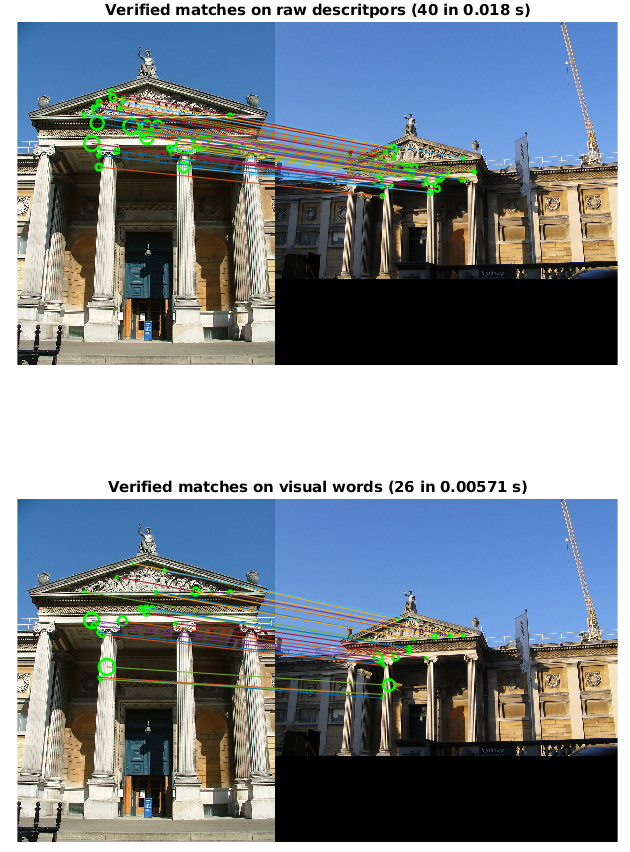
\includegraphics[width=0.5\linewidth]{IIIA_1}
		\caption{3.1x faster, with \( nnThreshold = 0.8\) and geometric verification}
		\label{fig:III_A1}
	\end{subfigure}

	\begin{subfigure}[b]{0.9\textwidth}
		\centering
		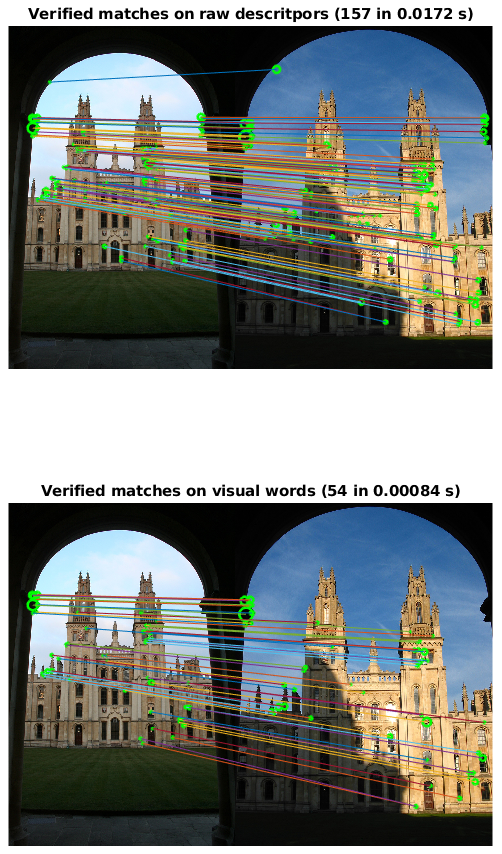
\includegraphics[width=0.5\linewidth]{III_A_11}
		\caption{20x faster, with \( nnThreshold = 0.8\) and geometric verification}
		\label{fig:III_A11}
	\end{subfigure}

	\caption{Accelerating descriptor matching with visual words between second neighbour test and geometric verification}
	\label{fig:III_A}
\end{figure}

This step is less important in practice because it's an individual step, which can be done seperatly from the query process, and the result of the translation into visual words can be easily stored with the image, as it represents nothing in comparaison with the size of the image.

\question{QIIIA.2: What is the speedup in seconds in searching a large, fixed database of 10, 100, 1000 images? Measure and report the speedup in seconds for 10, 100 and 1000 images.}

In Figure~\ref{fig:III_A}, the speedup in seconds per image in the databse is \( \approx 1.5~10^{-2}~s\), so, if the conjecture holds, for a database of 10, 100 and 1000 images respectively, the speedup would be \(0.15~s\), \(1.5~s\), \(15~s\).


\question{QIIIB.1: Why does the top image have a score of 1?}
The top image have such a score because it comes from the image database. So the histograms of visual words between the query and the same image in the databae are the same, hence the score of 1.

\question{QIIIB.2: Show the first 25 matching results, indicating the correct and incorrect matches. How many erroneously matched images do you count in the top results?}
The results of the search are presented in Figure~\ref{fig:IIIB}. The search took \( 7.51~10^{-6}~s/image\) and gives 9 correct answers over the 25 top results.

\singlefig{IIIB_2}{1}{Searching ashmolean\_000028 image in 660 images of the Oxford image database lite\_imdb\_100k}{fig:IIIB}

\question{QIIIC.1: Why is the top score much larger than 1 now?}
The score is now the number of inliers words between the query and the database. It's larger than 1 for the top result which shares every inliers words with himself.

\question{QIIIC.2: Illustrate improvements of retrieval results after geometric verification.}
\singlefig{IIIC}{1}{Searching ashmolean\_000028 image in 660 images of the Oxford image database lite\_imdb\_100k. Rescoring with number of inliers words}{fig:IIIC}
The result of the rescoring of the top 25 previous results is shown in Figure~\ref{fig:IIIC}. On the top 25 results, the 9 correct images are now ranked from 1 to 9,, with a score at least \( 4\) times bigger than the \(10\)th result.


\question{QIII.D: Full system}

\singlefig{IIID}{1}{Searching ashmolean\_000028 image in 660 images of the Oxford image database lite\_imdb\_100k. Rescoring with number of inliers words}{fig:IIIC}

\begin{figure}
	\begin{subfigure}[b]{0.9\textwidth}
		\centering
		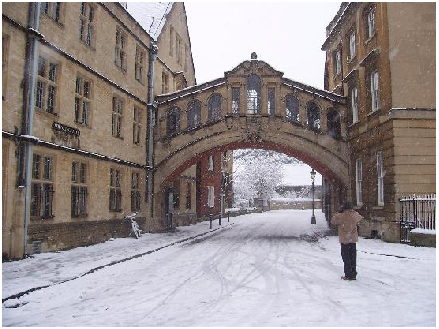
\includegraphics[width=1.\linewidth]{IIID_query}
		\caption{Quert image}
		\label{fig:III_D1}
	\end{subfigure}

	\begin{subfigure}[b]{0.9\textwidth}
		\centering
		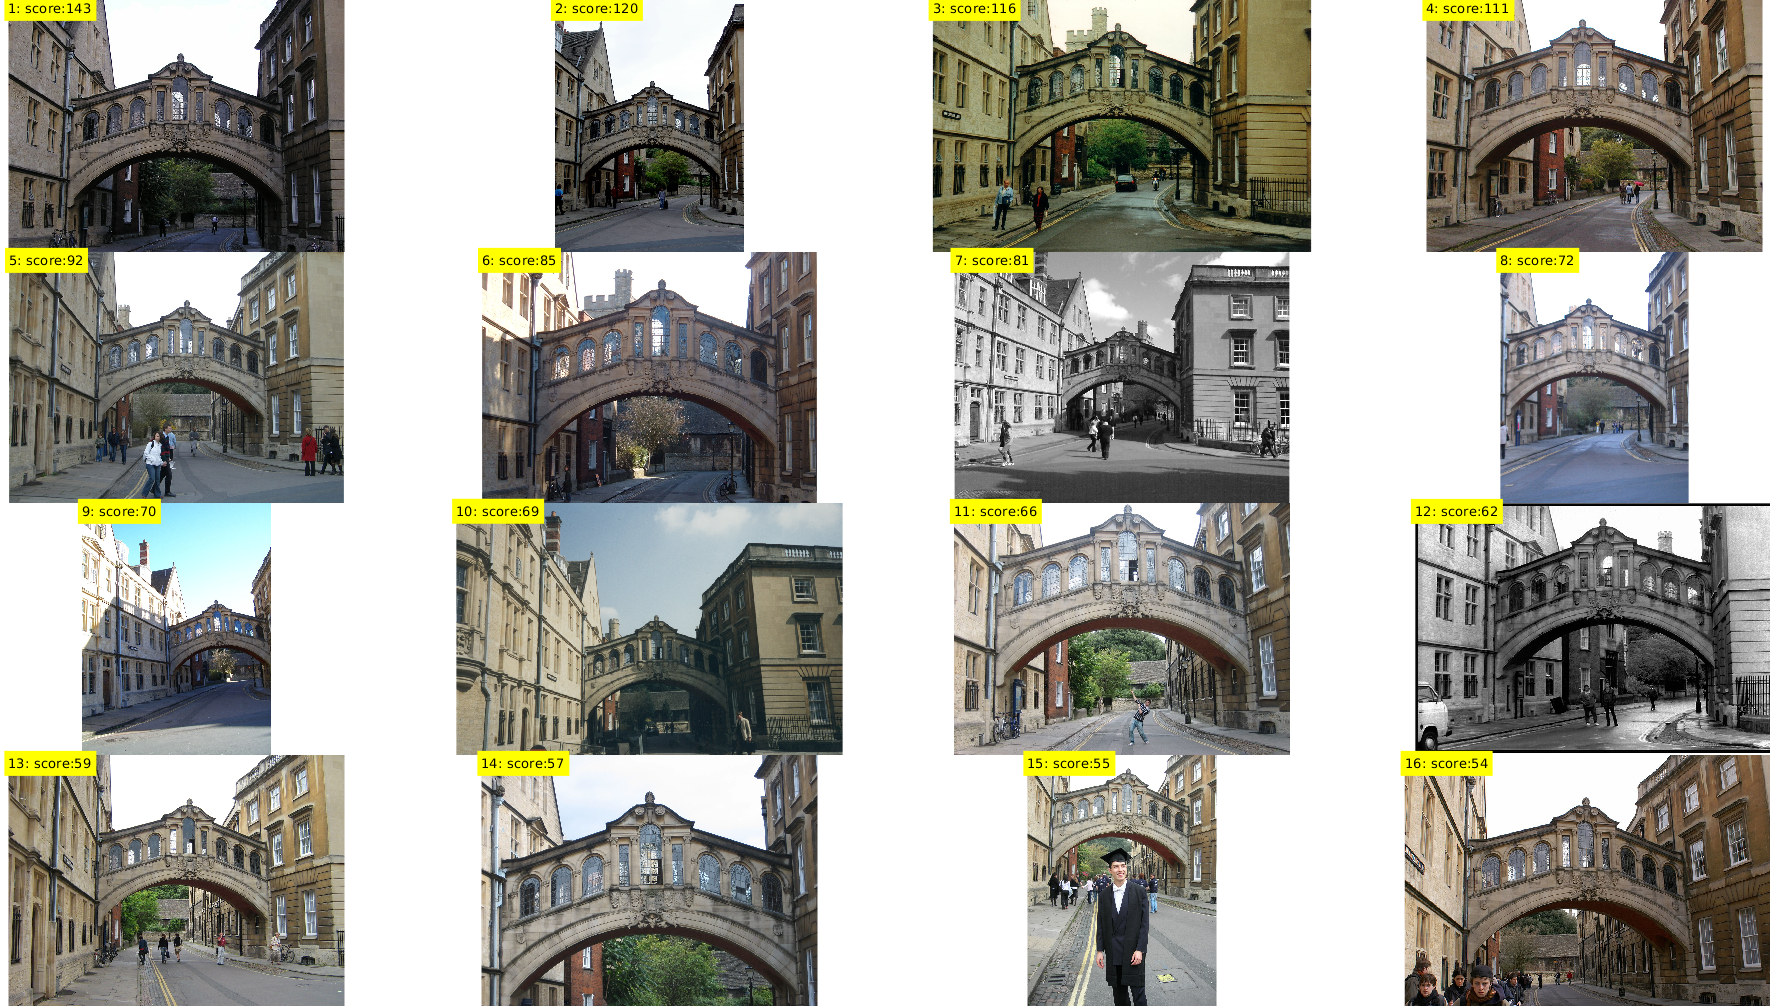
\includegraphics[width=1.\linewidth]{IIID}
		\caption{Top 25 results, rescoring with number of common visual words}
		\label{fig:III_D2}
	\end{subfigure}

	\caption{Searching mistery-building1 image in 660 images of the Oxford image database lite\_imdb\_100k with geometric rescoring}
	\label{fig:IIID}
\end{figure}


The query has yet not been shown to the database. The result of the search in the 660 images of the Oxford building database are shown in Figure~\ref{fig:IIID}. Over the top 25 results, only correct answers appear. The search took \(2.2~10^{-3}~s/image\) globally, but the index time was only \(6.1~10^{-3}~s/image\) as already computed in partIII.B.


\question{QIV.1: How many features are there in the painting database?}

\question{QIV.2: How much memory does the image database take?}

\question{QIV.3: What are the stages of the search? And how long does each of the stages take for one of the query images?}


\end{document}
